\chapter{SeL4}
Entrando adesso più nello specifico, si andrà ad approfondire quello che sarà il caso di studio di questa tesi e cioè \textit{seL4}. Nelle sezioni che seguiranno si avrà una panoramica completa del \textit{microkernel}, trattando singolarmente gli aspetti principali di quest'ultimo. Alla fine di questo capitolo si otterrà un quadro completo di com'è strutturato e delle sue capacità.

\section{Modello strutturale di seL4}
SeL4 \cite{sel4-whitepaper} fa parte della famiglia dei \textit{microkernel} L4 che risalgono alla prima metà degli anni '90, creato da Jochen Liedtke per sopperire alle scarse \textit{performance} dei primi sistemi operativi basati su \textit{microkernel}. SeL4 in particolare è stato sviluppato dal gruppo NICTA, oggi conosciuto con il nome di \textit{Trustworthy System}.
Come descritto nel capitolo precedente, essendo seL4 un \textit{microkernel}, ha un numero di righe di codice sorgente estremamente piccolo e questo è sufficiente per determinare che non è un sistema operativo, ma soltanto un \textit{microkernel}. Infatti non fornisce nessuno dei servizi che siamo solitamente abituati a trovare in un comune SO, "è solo un sottile involucro attorno all'hardware" \cite{sel4-whitepaper}. Tutti i servizi devono essere eseguiti in modalità utente e questi dovranno essere importati, ad esempio, da sistemi operativi \textit{open-source} come Linux (oppure scritti da zero). SeL4 è anche un \textit{hypervisor}, quindi è possibile eseguire macchine virtuali sulle quali far girare un comune SO, che fornirà i servizi non presenti in seL4.
Un esempio pratico è mostrato in Figura~\ref{fig:Virtualizzazione}, in cui è raffigurato seL4, una generica applicazione e due macchine virtuali (VM), sulle quali viene eseguita una versione ridotta al minimo di Linux (che quindi avrà poco più oltre al servizio che dovrà eseguire).
\begin{figure}[h]
  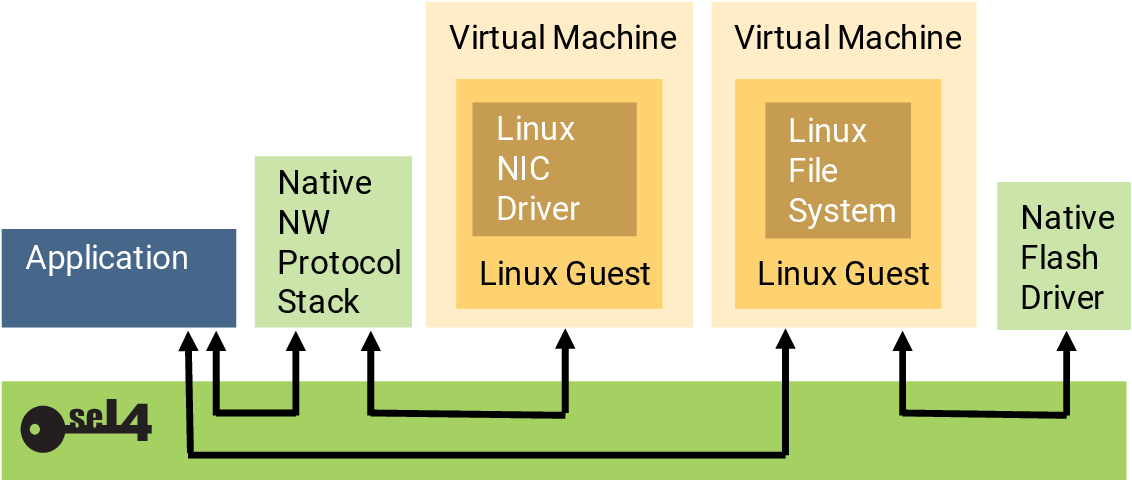
\includegraphics[width=\linewidth]{img/seL4Hypervisor.png}
  \caption{Virtualizzazione del SO Linux per l'integrazione dei servizi di \textit{networking} e \textit{file system}}
  \label{fig:Virtualizzazione}
\end{figure}
Queste due VM forniranno all'applicazione il servizio di \textit{networking} e il \textit{file system} per la gestione della memoria secondaria (\textit{hard disk}, supporti rimovibili, ecc.). Le comunicazioni tra le parti saranno gestite da un canale fornito dal \textit{microkernel}, ma le due macchine virtuali non avranno modo di comunicare tra di loro. Come si vede in figura, anche le comunicazioni tra le varie parti e l'applicazione sono ben delineate e precise: nessun'altra comunicazione al di fuori di quelle indicate dalle frecce è possibile.

\section{\textit{\uppercase{C}apability}}
Un concetto fondamentale in seL4 è quello di \textit{capability}, che è definita formalmente come un riferimento ad oggetto. Possiamo considerarla anche come un puntatore immutabile, cioè una \textit{capability} che farà sempre riferimento allo stesso oggetto.

SeL4 è un sistema \textit{capability-based} (basato sulle \textit{capability}): questo significa che l'unico modo per eseguire un'operazione è attraverso l'invocazione di una \textit{capability}. Ad ognuna di esse, inoltre, sono associati dei diritti di accesso: quindi una \textit{capability} è un incapsulamento di un riferimento ad oggetto con i diritti ad esso conferiti.
Per dare una definizione meno formale, si può pensare alle \textit{capability} come a delle chiavi di accesso estremamente specifiche riguardo su quale entità può accedere ad una particolare risorsa del sistema. Per di più, permettono di supportare il \textit{principle of least privilege}, principio del privilegio minimo chiamato anche \textit{principle of least authority} PoLA. Questo principio implica che ogni modulo deve avere accesso solo ed esclusivamente alle risorse strettamente necessarie al suo scopo.
In seL4 quindi i diritti dati ad un componente possono essere ristretti al minimo indispensabile per svolgere il loro lavoro, come richiesto dal PoLA, il che chiaramente è un grosso punto a favore per quanto riguarda la sicurezza.

Nei sistemi operativi più comuni tipo Windows o Linux l'accesso alle risorse è gestito dalle \textit{access-control list} (ACL). Quindi nel caso specifico di Linux, ad ogni \textit{file} viene associato un \textit{set} di \textit{bit}, che determinano quali operazioni (lettura, scrittura ed esecuzione) possono essere eseguite su di esso dai vari utenti (proprietario, gruppo e altri). Tutto ciò implica che ogni \textit{file} con lo stesso \textit{set} di permessi è accessibile ad uno specifico utente. Se ci si colloca nello scenario di voler avviare un programma, di cui non siamo sicuri dell'attendibilità, il quale abbia accesso ad uno e un solo \textit{file} specifico, questo non è possibile perché come può accedere a quel \textit{file}, può accedere anche a tutti gli altri che hanno associati gli stessi permessi.

Con le \textit{capability} questa eventualità non si può presentare perché il \textit{kernel} consentirebbe un'operazione se e solo se chi richiede di eseguire l'operazione ha la "giusta \textit{capability}" per eseguire l'operazione su quel \textit{file}. 

\subsection{Proprietà delle \textit{capability}}
Le \textit{capability} hanno la proprietà di interporsi tra chi crea una \textit{capability} e l'effettivo accesso ad una risorsa: questa proprietà prende il nome di \textit{interposition}. Se un utente dà una \textit{capability} ad un oggetto, esso non è in grado di sapere cosa effettivamente sia quell'oggetto, ma può chiaramente utilizzarlo anche senza sapere che tipo di oggetto sia.

Le \textit{capability} supportano la delega dei privilegi tra gli utenti: l'utente X ha un oggetto e vuole dare accesso ad esso anche all'utente Y; X può creare una nuova \textit{capability} e darla ad Y, senza conservare nessun riferimento all'utente X che l'ha creata. La nuova \textit{capability} può anche avere meno diritti di accesso (esempio solo lettura invece di lettura e scrittura) e inoltre X in qualsiasi momento può revocare l'accesso ad Y distruggendo la \textit{capability}. Questa seconda proprietà si chiama \textit{delegation}.

\section{\textit{\uppercase{H}ard \uppercase{R}eal-\uppercase{T}ime \uppercase{S}ystems}}
SeL4 è stato sviluppato in modo che possa essere utilizzato anche in casi in cui si sia in presenza di quelli che vengono chiamati \textit{hard real-time system}.
Un \textit{hard real-time system} è un sistema in cui il mancato rispetto di una scadenza può portare al fallimento dell'intero sistema. Un esempio molto comune e semplificato può essere l'autopilota di un'automobile. Un veicolo dotato di un \textit{software} di guida autonoma richiede la presenza di un numero estremamente elevato di sensori esterni ed interni al veicolo e il computer di bordo deve leggere, elaborare e dare una risposta immediata ad ogni minimo cambiamento di un valore proveniente da questi sensori. Se ad un certo punto l'elaborazione di un dato richiede più del tempo dovuto, anche solo di qualche millisecondo, c'è il rischio che questo comporti una serie  di ritardi a catena, che ad esempio causino il non rilevamento di un oggetto che si sta avvicinando al veicolo, oppure alla mancata correzione della traiettoria e quindi l'abbandono della carreggiata, con conseguenze anche catastrofiche.

SeL4 ha alcune caratteristiche che lo rendono adatto in ambiti \textit{hard real-time system}. Infatti, lo \textit{scheduling} dei processi in seL4 è basato sulla priorità. Il \textit{kernel} di sua iniziativa non cambierà mai la priorità di un processo, che è sempre decisa dall'utente.

Inoltre, quando seL4 esegue delle operazioni in modalità \textit{kernel} queste sono esenti da \textit{interrupt}. All'apparenza questo può sembrare grave se non fosse per il fatto che le chiamate di sistema sono tutte brevi. Solo la revoca di una \textit{capability} può richiedere tempi più lunghi, ma in presenza di queste operazioni seL4 adotta una politica di divisione dell'esecuzione in sotto operazioni più brevi. In aggiunta, ognuna di esse può essere annullata e poi ripresa da quel punto in poi, così da poter gestire degli eventuali \textit{interrupt} in attesa.

Questi due punti appena elencati sono caratteristiche fondamentali per gli \textit{hard real-time system}: \textit{scheduling} dei processi basato sulla priorità, che sia quindi facilmente analizzabile; latenza degli \textit{interrupt} limitata, essendo gli \textit{interrupt} disabilitati, non ci sarà nessuna latenza dovuta al cambio di contesto per gestire subito l'\textit{interrupt} e dato che le operazioni sono tutte brevi, questo non risulta essere un problema.
Per seL4 è stata eseguita una \textit{worst-case execution time} (WCET): questo vuol dire che è stato determinato un limite superiore di latenza di ogni \textit{system call} nel caso peggiore e ciò implica anche il caso peggiore di latenza di un \textit{interrupt}.

\subsection{\textit{Mixed-Criticality Systems}}
Un \textit{mixed-criticality system} (MCS) è un sistema costituito da più componenti che interagiscono tra di loro e che hanno differenti livelli di criticità. In questi sistemi è imperativo che il fallimento di un componente non influenzi gli altri componenti critici, e che questi siano quindi isolati e protetti dai componenti meno critici.

Un approccio classico per questo tipo di sistemi è isolare le criticità sia per quanto riguarda il tempo sia lo spazio. Ciò è noto come \textit{strict time and space partitioning} (TSP). Ma questo implica il dover assegnare staticamente l'area di memoria, il tempo di esecuzione e quindi lo \textit{scheduling}; per farlo si utilizzano dati misurati precedentemente nel caso pessimo. Essendo sistemi \textit{real-time}, ogni operazione deve avere dei limiti di tempo, quindi un'operazione su cui è stato misurato un tempo di esecuzione di 5 millisecondi (sempre nel caso pessimo) deve avere questa durata, non 4ms né tantomeno 6ms. Chiaramente, determinando staticamente i tempi e gli spazi nel caso peggiore, si è sicuri che questi vengano rispettati. C'è da considerare però che non sempre si presentano dei casi pessimi e si ha quindi uno scarso utilizzo delle risorse; per di più la latenza di un \textit{interrupt} nel caso pessimo, può essere molto costosa.

SeL4 supporta i \textit{mixed-criticality system}. Per quanto riguarda l'isolamento, si è già visto che le \textit{capability}, in termini di spazio, intrinsecamente lo garantiscono. Resta perciò da esaminare il comportamento da un punto di vista temporale.

Il \textit{microkernel} normalmente utilizza due parametri per gestire lo \textit{scheduling} dei processi: la priorità e la quantità di tempo. La priorità determina l'ordine di esecuzione dei processi, mentre il \textit{time slice} (quanto di tempo) determina per quanto tempo il \textit{kernel} lascerà in esecuzione un \textit{thread}, prima di fermarlo per selezionare un altro processo. Quest'ultimo verrà scelto tra i processi pronti in base alla priorità, con una politica \textit{round-robin} tra i pari livelli di priorità.

La versione MCS di seL4 si comporta diversamente. L'accesso al processore viene controllato dalle \textit{capability}, un componente può ottenere la CPU solo se ha una \textit{capability} che glielo permette e il tempo di esecuzione è codificato in essa. Tale politica si chiama \textit{scheduling-context \textit{capability}}. Quest'ultimo contiene due attributi principali: 
\begin{enumerate}
	\item \textit{time budget}, che sostituisce il \textit{time slice};
	\item \textit{time period}, che determina invece quante volte un \textit{budget} può essere usato per periodo, evitando in questa maniera che un processo monopolizzi la CPU, indipendentemente dalla sua priorità.
\end{enumerate}

\section{Sicurezza e \textit{performance}}
Come già detto nelle prime righe di questo capitolo, la famiglia dei \textit{microkernel} L4 nasce per sopperire alle scarse \textit{performance} dei suoi predecessori. Finora è stato descritto il funzionamento generale di seL4, con particolare attenzione sulla sicurezza di questo sistema. Chi è dell'ambito, sa già che spesso sicurezza e buone prestazioni non vanno molto d'accordo. Garantire la sicurezza vuol dire attenersi a regole ben precise e controlli, che spesso poi portano a rallentamenti e quindi vanno ad influire sulle \textit{performance} di un sistema. È di conseguenza lecito domandarsi se questo \textit{microkernel} sia performante o meno.

Nonostante non fosse nelle prerogative dello sviluppo di seL4, questo alla fine, si è rivelato il più performante dei \textit{microkernel} della famiglia L4. Inoltre sono state scritte altre pubblicazioni indipendenti, che mettono a confronto seL4 con altri \textit{microkernel}, per studiarne le \textit{performance}, in particolare Fiasco.OC, Zicron e CertiKOS. Confrontando i costi dell'IPC si può vedere che seL4 ha un bel vantaggio, anche di oltre un fattore 2, rispetto agli altri \textit{microkernel}.
Gli articoli che mostrano gli studi delle \textit{performance} sono riportati in \cite{skybridge} per quanto riguarda il confronto tra Fiasco.OC, Zicron e seL4, mentre in \cite{CertiKOS}, si trova il confronto fra CertiKOS e seL4.